% Metódy inžinierskej práce

\documentclass[10pt,twoside,slovak,a4paper]{article}

\usepackage[slovak]{babel}
%\usepackage[T1]{fontenc}
\usepackage[T1]{fontenc} % lepšia sadzba písmena Ľ než v T1
\usepackage[utf8]{inputenc}
\usepackage{graphicx}
\usepackage{url} % príkaz \url na formátovanie URL
\usepackage{hyperref} % odkazy v texte budú aktívne (pri niektorých triedach dokumentov spôsobuje posun textu)
\usepackage{todonotes}
\usepackage{cite}
% \usepackage{fancyhdr}
\usepackage{wrapfig}
\usepackage{stfloats}
%\usepackage{times}

% \pagestyle{fancy}
% \fancyhead{}



\title{Je odporúčací systém Netflix-u problém ?\thanks{Semestrálny projekt v predmete Metódy inžinierskej práce, ak. rok 2024/2025, vedenie: Mgr. Yevheniia Kataieva, PhD.}}

\author{Adam Glogovský\\[2pt]
	{\small Slovenská technická univerzita v Bratislave}\\
	{\small Fakulta informatiky a informačných technológií}\\
	{\small \texttt{xglogovsky@stuba.sk}}}

\date{\small 5. október 2024} 


\begin{document}

\maketitle
\begin{abstract}
	Cieľom tejto práce je analyzovať, ako spoločnosť Netflix spracúva užívateľské informácie a posúdiť, či je tento proces správny. Na úvod objasním problematiku všeobecných odporúčacích systémov, ktoré slúžia ako základ pre pochopenie kontextu. Následne sa zameriam na to, kam Netflix posiela užívateľské informácie, akým spôsobom ich spracúva a ako tieto dáta využíva na zvýšenie užívateľského komfortu na platforme. Zároveň preskúmam, či takéto zlepšenie užívateľského zážitku znamená zvýšené náklady pre platformu a či je tento proces efektívny a finančne prospešný pre Netflix.

	Veľká pozornosť bude venovaná analýze spôsobu spracovania údajov. Poukážem na etické aspekty tohto procesu a preskúmam, či je správne tieto informácie spracúvať daným spôsobom. Kľúčovým prvkom, na ktorý sa zameriam, je algoritmus, ktorý spracúva užívateľské dáta, a infraštruktúra, v ktorej tento proces prebieha.\cite{amatriain2015recommender}

	Ďalej sa budem zaoberať otázkou, či algoritmy Netflixu neznevýhodňujú menej populárny alebo „nemainstreamový“ obsah tým, že ho menej zobrazujú užívateľom. Preskúmam, či je tento obsah iba menej favorizovaný a posúvaný nižšie v poradí vyhľadávania, alebo je pre určitých užívateľov úplne skrytý.

	Na záver tejto práce získate prehľad o tom, ako Netflix spracúva užívateľské informácie, posúdenie etickej správnosti tohto procesu, jeho profitabilitu pre spoločnosť a jeho vplyv na užívateľov platformy.\cite{OpenAI_ChatGPT}
\end{abstract}

\section*{Úvod}
Zaujímalo vás niekedy, ako Netflix určuje, čo by sa vám pravdepodobne páčilo keď prechádzate cez ich ponuku filmov a seriálov ? Viac o tejto tématike sa dozviete tu: \ref{Algoritmus}. Alebo ako určuje kde a ako tieto filmy a seriály rozložiť na hlavnú stránku ? Viac o tomto tu:\ref{Krátka pozornosť}. Možno vás niekedy zaujímalo či je takýto algoritmus profitabilný a prečo vlastne chce Netflix zlepšiť svojim používateľom používanie ich platofrmy ? Odpoveď nájdete tu:\ref{Profit}

\newpage

\section{Krátka história} \label{Netflix cena} %viac o minulosti a o netflix prize
Už v roku 2006 mal Netflix záujem o odporúčacie systémy.\cite{amatriain2015recommender} Preto, oznámil Cenu Netflixu ako súťaž strojového učenia o to, kto vytvorí aspoň o 10\% lepší odporúčací systém ako bol ten ich, Cinematech. Nový odporúčací systém mal byť lepší v konkrétne \textit{RMSE(root mean squared error)}\footnote{RMSE - root mean squared error - odmocnina priemerného rozdielu medzi reálnymi a očakávanými hodnotami\cite{EncyclopaediaBritannica}} pre predpokladané hodnotenie. A zrazu sa veľmi veľa rozdielnych firiem snažilo zlepšiť svoje algoritmy.
%uz za tyzden ich prekonali, treba najst zdroj

\section{Problem zlatej rybky} \label{Krátka pozornosť}
Keď majú ľudia príliš veľa vecí, na ktoré sa môžu pozrieť, nepozrú sa na nič. Štúdia spomenutá v \cite{10.1145/2843948} zistila, že v priemere typický používateľ stráca pozornosť po pribižne minúte prezerania si možností, čo si pozrie. No a teda sa Netflix veľmi usiluje aby počas tejto minúty, ukázal užívateľovi čo najlepší výsledok. Určite sa aj vám niekedy stalo, že ste otvorili Netflix hlavnú stránku, chvíľku popozerali a potom Netflix vypli. To je pre Netflix najhoršia vec, čo môže nastať, pretože vy ste si nič nepozreli a aj napriek tomu, že im platíte mesačne, ak sa toto stane viac krát, určite to predplatné zrušíte. Nikto predsa nechce službu ktorá im neponúka to, čo chcú.

\section{Algoritmus} \label{Algoritmus}
Ak človek nemá žiadne odporúčanie od kamaráta alebo známeho, je odkázaný prehľadávať veľké množstvo filmov a seriálov, o ktorých nevieme či sú dobré alebo nie. Jednoducho si o každom z filmov alebo seriálov dokážeme dohľadať hodnotenia a žánre, ale nikdy nevieme, či sa to bude páčiť práve nám. A preto prichádzajú "na scénu", veľmi potrebné algoritmy ktoré vďaka veľkému množstvu dát dokážu predpovedať ako veľmi sa nám bude daná šou páčiť, ukázať nám hodnotenia ľudí podobnej filmovej chute ako my a dokonca aj predpovedať aké hodnotenie jej dáme. ''V Netflixe nieje jeden model ktorý poháňa všetky odporúčania ale skôr set techník ktoré sa navzájom prepájajú v rovnakom cieli - zvýšiť užívateľskú spokojnosť''\cite{Steck_Baltrunas_Elahi_Liang_Raimond_Basilico_2021}. No a teda aké všetky algoritmy vlaste používa Netflix na svojej platforme ? Viac sa dozviete v najbližších podsekciách\ldots
\begin{figure}
	\begin{center}
		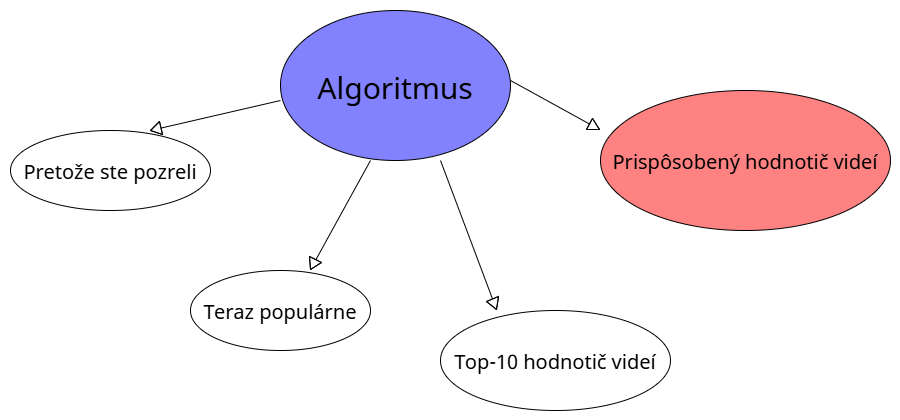
\includegraphics[scale=.4]{DiagramAlgoritmus.png}
		\caption{Diagram popisujúci rozdielne časti algorimtmu}
	\end{center}
\end{figure}

\subsection{Prispôsobený hodnotič videí}
Na hlavnej stránke môžte vidieť naozaj veľa filmov a seriálov. Sú ale rozdelené do riadkov, vždy podľa toho čo ich spája. Pre uvedenie príkladu, riadok komediálnych filmov sa pre nás vytvorí, ak sme si niekedy predtým pozreli nejakú komédiu. Samozrejme sa to odvíja od toho, aký člen domácnosti práve pozerá, tak isto od toho aké hodnotenie dal danej komédií a tak isto ako dlho ju pozeral a koľko takých komédií si pozrel. Na všetkom z tohto pracuje \textit{PVR(Personalised Video Ranker)}\footnote{PVR - personal video ranker - Prispôsobený hodnotič videí\cite{10.1145/2843948}}\cite{10.1145/2843948}
\subsection{Top-N hodnotič videí}
Iný typ riadku ktorý je tiež na hlavnej stránke ale ukazuje trošku niečo iné. Jeho cieľ je taký istý - ukázať užívateľovi najlepší obsah. Pre zmenu, to teraz nefiltruje podľa iba určitého žánru ale z celého katalógu nám ukazuje to najlepšie čo bol schopný nájsť pre daného užívateľa a ukáže prvých 10, inokedy viac, odporúčaní, ktoré sú na začiatku ''listu'' ktoré vytvára tento algoritmus.\cite{amatriain2015recommender}
\subsection{Teraz populárne}
Tento algoritmus je veľmi jednoduchý. Keďže nezohľadňuje takmer žiadnu personalizáciu, je najčastejšie používaný na začiatku resp. pre nových používateľov. Jeho hlavný zmysel je, ukázať obsah ktorý je práve populárny v danom ročnom období alebo časti roka. Tak isto môže zohľadnovať polohu a teda uprednostňovať obsah napr. zo Slovenska atď..
\subsection{Pokračujte v pozeraní}
Keďže je veľmi dôležité ukladať pokrok pozerania seriálov alebo filmov na pokračovanie, tento riadok je veľmi potrebný. Aj prvky v tomto riadku sú usporiadavané pomocou vlastného algoritmu, tento algoritmus zohľadňuje čas ktorý ubehol od posledného pozretia daného obsahu, alebo aj či užívateľ pozrel podobný obsah.


\section{Profitabilnosť} \label{Profit}
Netflix má približne 235 miliónov platených užívateľov a úspech Netflixu vykvetol hlavne vďaka tomu, že začali používať vyššie spomenuté algoritmy skôr ako konkurencia.
Keďže 80\% sledovania na platforme tvorí sledovanie odporúčaného obsahu práve predtým spomenutými algoritmami, tak to znamená, že fungujú veľmi dobre a, že sa im vyplatia \cite{pub.1158091188}. V podstate bez ohľadu na to, koľko by ich to stálo, vyplatí sa im udržiavať a vyvíjať tieto algoritmy. Keďže za prehrávanie určitého obsahu, či už populárneho a dobre hodnoteného alebo nepopulárneho a menej dobre hodnoteného, platí Netflix prakticky tú istú sumu a teda im je to v podstate jedno, čo užívateľovi zobrazí, jediné na čom záleží je, že si to užívateľ pozrie, je spokojný a príde na platformu znova. \cite{amatriain2015recommender}

Pre jednoduché porovnanie odporúčacieho systému Netflixu s napr. Spotify odporúčacím systémom. Môžme vidieť veľmi veľký problém v tom, že Spotify uprednostňuje populárnu hudbu a obsah oproti tomu menej populárnemu , pretože z toho má vačší profit a teda je stavaný aj ich odporúčací systém okolo profitu\cite{10425661}. Keďže každá firma chce mať profit, je to v pochopiteľné, ale problém je, že potom sú utláčaní nepopulárny umelci a majú problém vytvoriť zisk. Na rozdiel od Spotify, Netflix profituje za všetok obsah rovnako, je menej podstatné uprednostňovať populárny obsah. O tom, že Netflix je na tom finančne veľmi dobre a raste aj nadalej oproti minulým rokom, hovorí aj ich výročná správa o profite\cite{AnnualReportNetflix2023}.
\begin{center}
	Peňažná bilancia zisku Netflixu:
	\vspace{0.2cm}

	\begin{tabular}{||c | c||}
		\hline
		Dátum      & Čistý zisk   \\ [0.5ex]
		\hline\hline
		31.12.2020 & 7,57 Mld \$  \\
		\hline
		31.12.2021 & 12,69 Mld \$ \\
		\hline
		31.12.2022 & 17,18 Mld \$ \\
		\hline
		31.12.2023 & 22,59 Mld \$ \\
		\hline
	\end{tabular}
	\cite{AnnualReportsNetflix}
\end{center}
Tento profit sa odvíja aj na hodnote ich akcie, tá bola v 01. novembra 2023 iba 420,19\$ ale tohto roka v ten istý dátum sa vyšplhala na neuveriteľných 756,10\$ za akciu. To je zvýšenie o takmer 80\% za jeden rok.\cite{StockValueNetflix} A tak isto ich peňažná bilancia.

\begin{center}

	Enormný rozdiel hodnoty akcie Netflixu:

	\begin{tabular}{|c | c|}
		\hline
		Dátum      & Hodnota    \\ [0.5ex]
		\hline\hline
		01.11.2023 & 420,19  \$ \\
		\hline
		01.11.2024 & 756,10 \$  \\
		\hline
	\end{tabular}
	\cite{StockValueNetflix}
\end{center}

\section{Rozloženie hlavnej stránky} \label{Rozloženie}
Keďže už sme si popísali ako fungujú algoritmy, teraz si môžme popísať ako personalizovaný obsah rozkladá na stránku. Ako už predtým bolo spomenuté, užívateľ má krátku dobu pozornosti a Netflix preto rozdeľuje tento obsah do riadkov hneď na hlavnú stránku. Treba si ale uvedomiť že Netflix je zväčša používaný v domácnostiach a teda do napr. top 10 sa snaží dávať obsah ktorý si užije napr. otec, mama a ďalší členovia rodiny. Tak isto sa snaží nájsť položku pre celú rodinu. Ak je rodina jednočlenná, tak sa snaží nájsť výber z rozdielnych nálad a záľub daného užívateľa ktoré zisťujú dané algoritmy.\cite{amatriain2015recommender}

Netflix chce aby sme vedeli, ako sa ich systém adaptuje našej chuti. Tak isto sa snaží vybudovať dôveru v tieto odporúčania a tiež sa snaží vysvetliť prečo by sme si to chceli pozrieť. Toto reprezentuje popisok k danemu filmu/serialu, tak isto to ukazuje predikciu hodnotenia ake by sme dali danému filmu/seriálu.

\section{Porovnanie HBO Max a Netflix} \label{Porovnanie}
Kým Netflix sa snaží používať rozličné počítačové algoritmy a predikcie hodnotení ktoré získává z našich akcií na platforme spomenutých v predchadzajúcich sekciách. Tak HBO Max sa snaží uchovať si iný prístup, a to tak, že implementuje aj ľudsky vybraný obsah. Tento prístup je podľa nich kľúčový k úspechu. A do budúcna, sa budú snažiť ešte viac zvýšiť tento ľudský dotyk pri výbere obsahu. A teda tento model odporúčania je bližšie k odporúčaciemu systému Spotify než Netflix. \cite{Arman1701480}
Pre číselné porovnanie, Netflix má, ako už bolo spomenuté, 235 miliónov užívateľov, HBO Max má približne 73 miliónov. Veľkosť knižnice seriálov a filmov pre Netflix je 5831 a pre HBO Max to je 3235. \cite{Arman1701480} Keďže akcie HBO niesú verejne predajné, a samotný profit z HBO je zaštítený pod Warner Bros, nedostal som sa k dôveryhodným informáciám o profite z HBO Max.\cite{WarnerBrosHBO}

Ale ak porovnáme známe čísla používateľov a knižnice, dokážeme si vyvodiť porovnanie týchto konkurenčných firiem. Všimnúť sme si mohli, že Netflix má oveľa viac používateľov, pravdepodobne je to vďaka algoritmom ktoré očividne fungujú, ale tak isto, to môže byť tým, že Netflix, je na trhu oveľa dlhšie a teda, ak u ľudí vyvolal spokojnosť, ľudia nemajú potrebu skúšať nové platformy. To znamená, že Netflix, robí dobrú prácu s udržiavaním si užívateľov. Tak isto je ale dôležité podoknúť, že relatívne nová služba v porovnaní s Netflixom, dokázala za takú krátku dobu, získať tretinu používateľov ktorý používajú Netflix. Tak isto treba poznamenať, že veľké percento z týchto užívateľov pravdepodobne používa obe tieto platformy a teda sú v štatistike započítaní dva krát.

\section*{Záver}

Touto prácou som prišiel na to, že odporúčací systém Netflixu, je veľmi komplexný, spolieha sa na niekoľko algoritmov, ktoré implementuje priamo do svojej stránky.

Porovnaním Netflixu s ďalšími platformami, som zistil, že ich systém, je veľmi efektívny, a v praxi funkčný. Iné platformy sa snažia vytvárať vlastné systémy a meniť ich originálne. Podľa čísel, je Netflix ale stále najpoužívanejší.

Taktiež analýzou samotného odpourúčacieho systému Netflixu, som prišiel na to, že zbiera množstvo informácií od užívateľov, ale mal by ich používať len pre zlepšenie používateľovho zážitku na platforme. Samozrejme podľa výročných správ som prišiel na to, že rast samotnej firmy je kladný a teda môžme usúdiť, že je to tak, aj vďaka odporúčaciemu systému.

Pokračovaním práce by mohlo byť spracovanie hlbšej analýzy rozličných algoritmov ako Netflixu, tak aj ďalších platforiem a ich porovnanie. Zaujímavé by bolo zistiť ako veľa údajov u užívateľov sa ukladá a ako veľa sa reálne použije nevinne.


% týmto sa generuje zoznam literatúry z obsahu súboru literatura.bib podľa toho, na čo sa v článku odkazujete
%\begin{figure}
\bibliography{literatura}
\bibliographystyle{abbrv} % prípadne alpha, abbrv alebo hociktorý iný
%\end{figure}

\end{document}
